\section*{Problem 1.6}

$$\tau = -\mathbf{K}_d \tilde \omega - k_p \tilde \epsilon $$
$$\tilde \omega = \omega - \omega_d $$
\\ $\omega_d $ is given by the reference signals from the previous problem, $\phi(t) = 10 \sin{(0.1t)}, \theta(t) = 0, \psi(t) = 15 \cos{0.05t}$.
\\ We will be using equation (2.26) in Fossen:
$$ \omega_d = \mathbf{T}_{\Theta_d}^{-1}(\Theta_d) \dot \Theta_d $$
$$ \omega_d = \m{\dot \phi \\ 0 \\ 0} + \mathbf{R_{x, \phi}^\top} \m{0 \\ \dot \theta \\ 0} + \mathbf{R_{x, \phi}^\top} \mathbf{R_{y, \theta}^\top} \m{0 \\ 0 \\ \dot \psi} $$
$$ = \m{\cos{(0.1t)} \\ 0 \\ 0} + \m{1 && 0 && 0 \\ 0 && c\phi && s\phi \\ 0 && -s\phi && c\phi} \m{c\theta && 0 && -s\theta \\ 0 && 1 && 0 \\ s\theta && 0 && c\theta} \m{0 \\ 0 \\ -0.75 \sin{0.05t}}$$
$$ = \m{\cos{0.01t} - \sin\theta \cdot 0.75 \sin{0.05t} \\ \cos \theta \sin\phi \cdot 0.75 \sin{0.05t} \\ \cos \theta \cos \phi  \cdot 0.75 \sin{0.05t} } $$



\begin{figure}
    \centering
    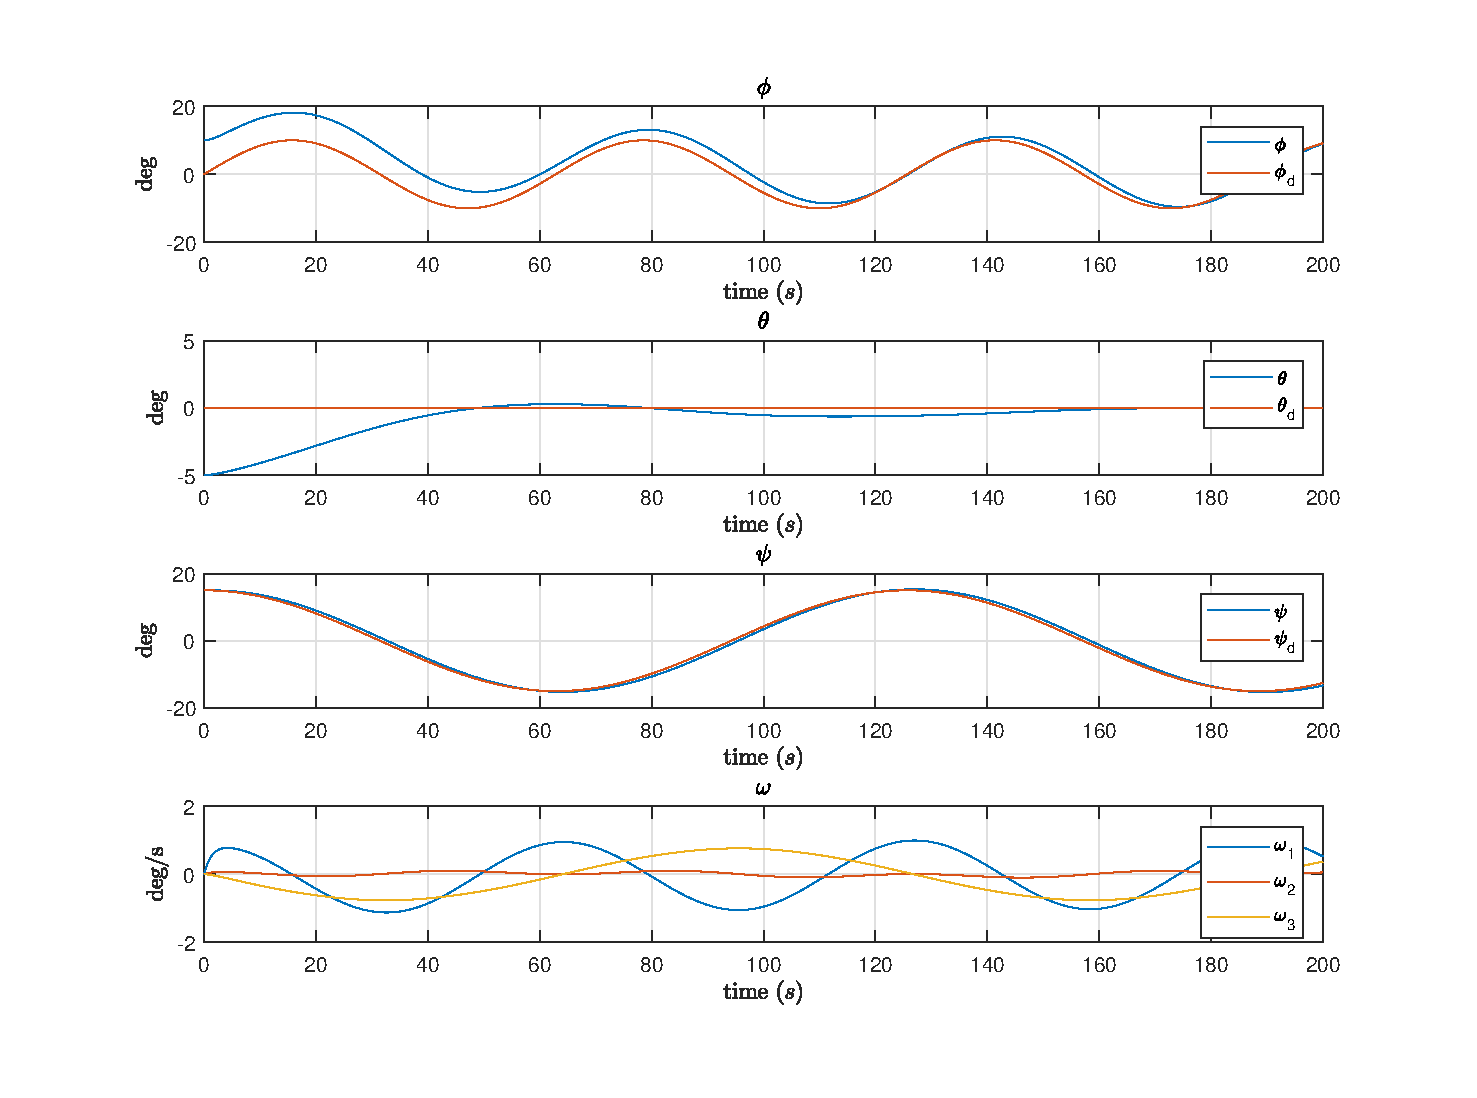
\includegraphics[scale=0.8]{eulang3.eps}
    \caption{Euler Angles Simulation}
    \label{fig:eulang3}
\end{figure}


\begin{figure}
    \centering
    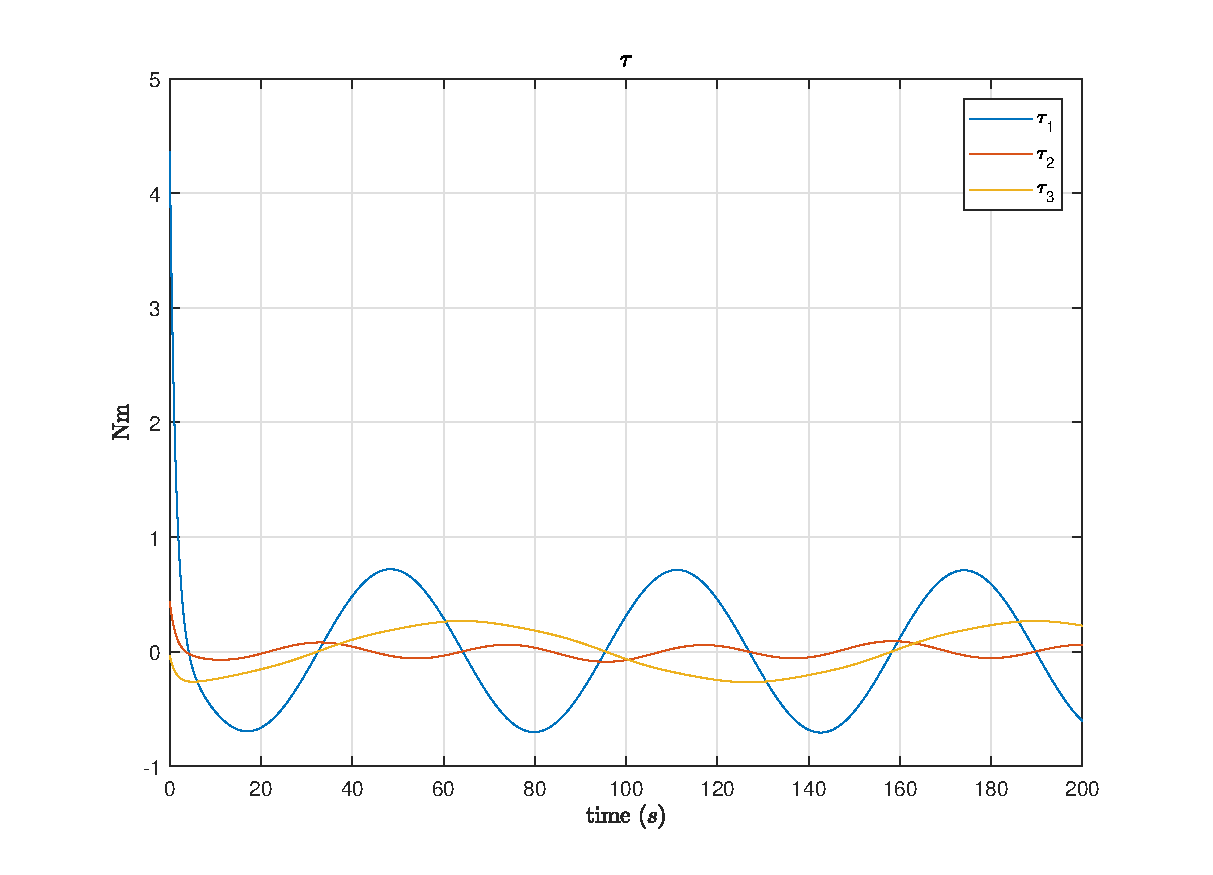
\includegraphics[scale=0.8]{tau3.eps}
    \caption{Euler Angles Simulation}
    \label{fig:tau3}
\end{figure}



\begin{figure}[h!]
    \centering
  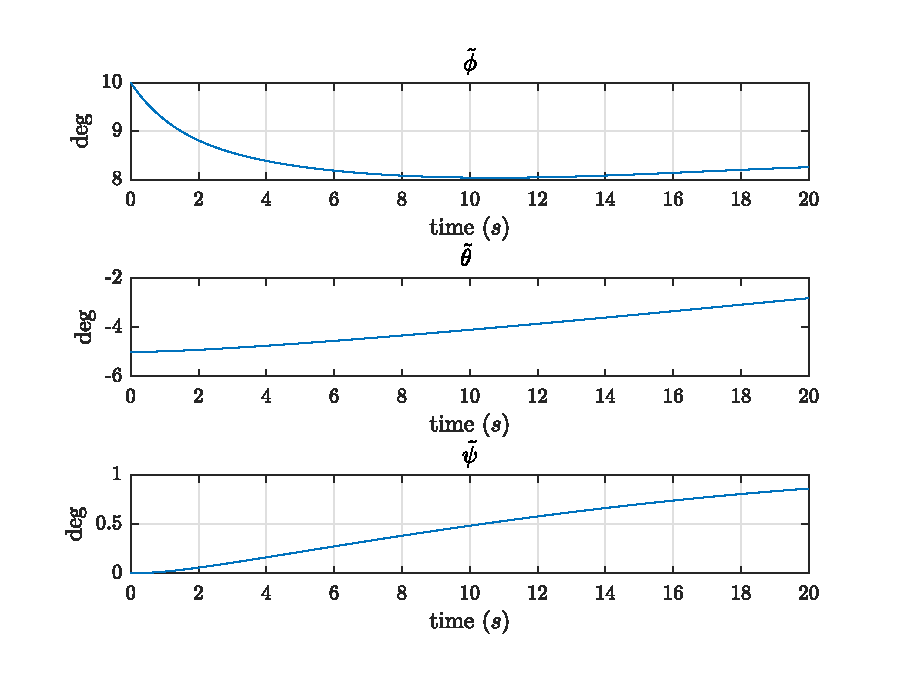
\includegraphics[scale=0.8]{eulang_tilde.eps}
  \caption{Euler angles tracking error}
  \label{fig:eulang:tilde1}
\end{figure}